\documentclass{csse4400}

\usepackage{CJKutf8}

\title{Scalable Data Analysis}
\author{Brae Webb}
\date{Semester 1, 2022}

\begin{document}
\maketitle

\section*{Summary}
In this assignment, you will demonstrate your ability to \textsl{design},
\textsl{implement}, and \textsl{deploy} a web application which can handle a high load,
i.e. a scalable application.
You'll be asked to deploy a tool where researchers upload text data (a \textsl{corpus}),
your service will analyse the corpus and provide the researcher with information to assist them in understanding the corpus.
Specially you need to support:
\begin{itemize}
    \item Uploading a large corpus (order of gigabytes).
    \item Perform analysis techniques on the data while remaining responsive to the user.
    \item Present the results in a human-readable format, as well as making the results available via a pre-specified API.
\end{itemize}

Your service will need to be deployed to AWS and will undergo automated load-testing to ensure it meets the required scalability.

\section{Introduction}
The world today is full of data.
For years, tech companies have been collecting data by default without having an immediate use for the data.
The explosion of interest in fields such as AI and machine learning can be attributed to the availability of these large collections of data.

\begin{figure}[ht]
  \begin{center}
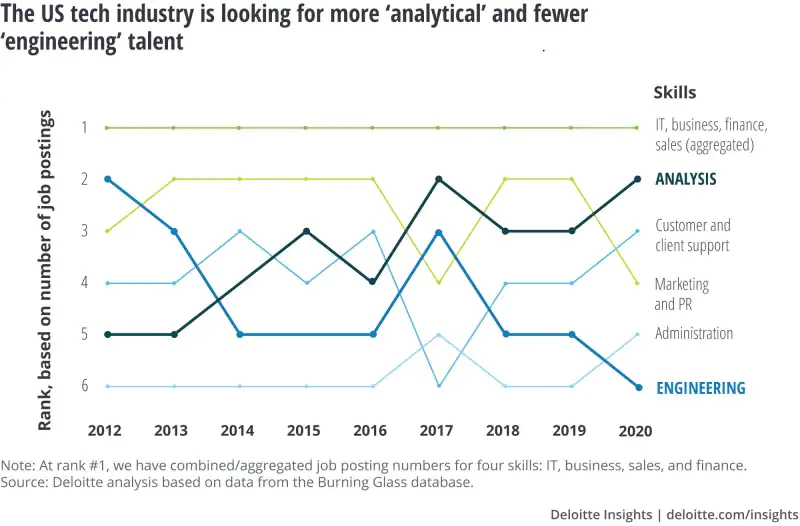
\includegraphics[width=0.6\textwidth]{analysis-demand}
  \end{center}\caption{Increasing demand for data analysts in the US \cite{data-analysis-shortage}.}
\end{figure}

\paragraph{Importance of Explainability}
Something which is becoming increasingly apparent to machine learning researchers is the demand for machine learning models to be \textsl{explainable}.
An interesting demonstration of what can go wrong without \textsl{explainability} is COVID-Net~\cite{covidnet}.
Researchers explored the applicability of machine learning models to detecting COVID-19 from chest X-rays.
The results were quite promising, the researchers were reportedly able to detect the virus with a high degree of accuracy.
Unfortunately (or rather fortunately), later research utilizing explainability techniques indicated that the developed model takes shortcuts~\cite{covidnet-debunk}.
They demonstrate that the results of the model are highly dependant on artefacts in the X-ray which indicate external factors.
For example, the model may associate patients scanned with a portable X-ray with a higher likelihood of having the virus as it may indicate the severity of their situation.

\begin{figure}[ht]
  \begin{center}
    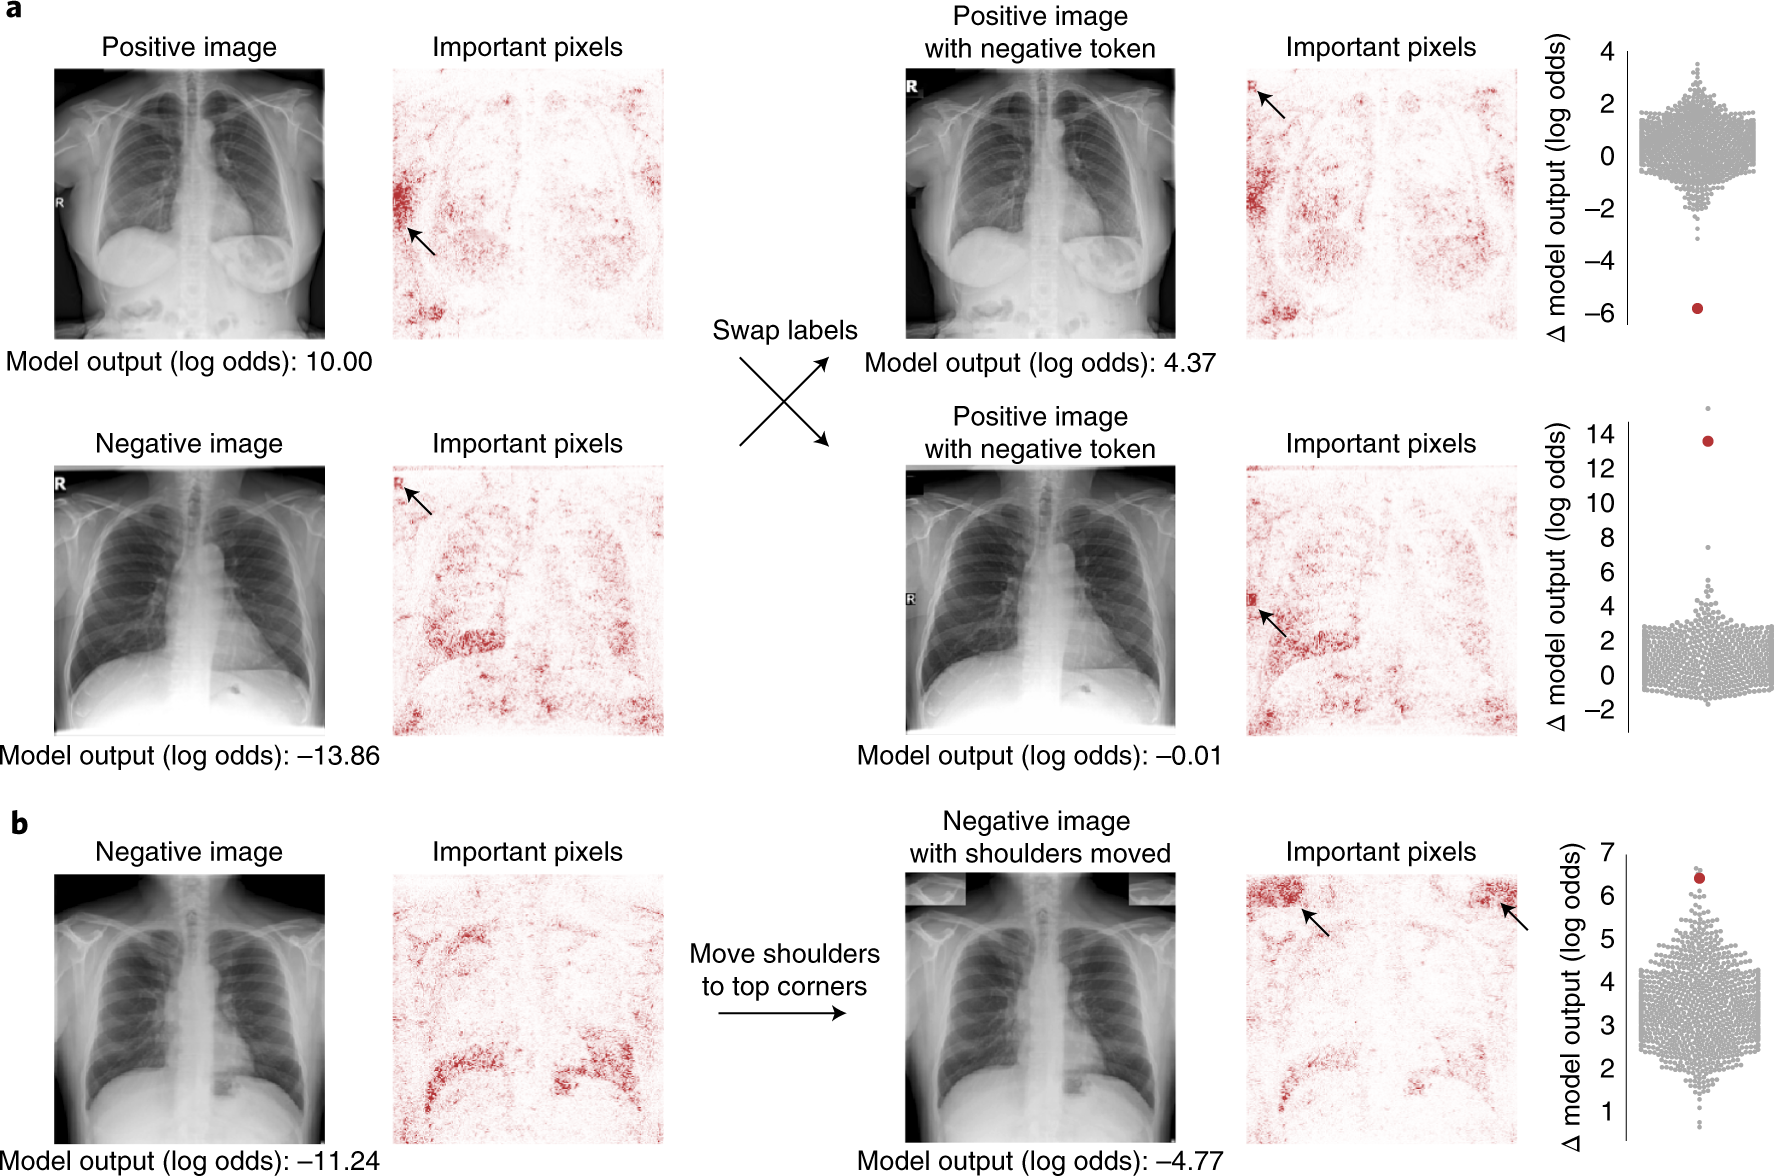
\includegraphics[width=0.8\textwidth]{covidnet-markers}
  \end{center}
  \caption{Experimental confirmation of insights from saliency maps and CycleGANs via radiograph modification~\cite{covidnet-debunk}.}
\end{figure}

\paragraph{Your Task}
For this assessment, you'll be assisting machine learning researchers in the development of a Exploratory Data Analysis (EDA)
(sometimes called \textsl{pre-modelling explainability}) tool.
Specifically, you will need to develop a web interface which allows researchers to upload text data which they wish to use for
Natural Language Processing (NLP) research.
Your software will perform a number of EDA techniques on the data and present the results to the researchers once complete.
The challenge is that often NLP corpuses can be quite large.
A researcher may upload Amazon's entire product review collection totalling 34GBs~\cite{amazon-reviews}.
Your software is expected to remain available and usable to other users while that data is processing.

\section{Features}
You are expected to implement the following features to analyse the uploaded data.
Features are given in order of increasing inefficiency for a computer,
making scaling more challenging.
Implementing only some of the listed features will still be worth marks, see the marking criteria at the end of the sheet.

Calculate/compute and display the following:
\begin{itemize}
    \item the total size of the uploaded data;
    \item the total amount of words;
    \item aggregate statistics of the length of words;
    \item a histogram of the length of words;
    \item a word cloud of most frequently used words; and
    \item TODO sentiment analysis.
\end{itemize}

\section{Interface}
Based off Evan's solution.

\section{Submission}

\section{Criteria}

\section{Academic Integrity}

\bibliographystyle{ieeetr}
\bibliography{references}

\end{document}